\section{Deployment Environment}\label{sec:env}

\subsection{Local containerised cluster}
\Cref{fig:topology} shows the whole system. One master and up to four workers run as Docker
containers on a single host, connected by a user-defined bridge network in which each
container is reachable by its host name. The host and container specifications are
given in \cref{tab:env}.

\begin{figure}[t]
\centering
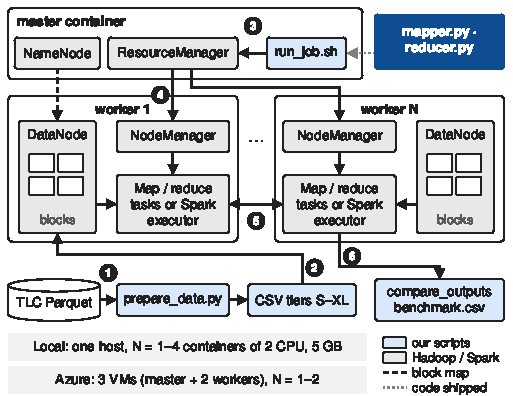
\includegraphics[width=\columnwidth]{figures/overview.pdf}
\caption{System overview. \textcircled{\scriptsize 1}~TLC Parquet files are cleaned
into CSV tiers and \textcircled{\scriptsize 2}~written to HDFS, whose 128\,MB blocks
are spread over the $N$ workers. \textcircled{\scriptsize 3}~\texttt{run\_job.sh}
submits a job to the ResourceManager, which \textcircled{\scriptsize 4}~starts map and
reduce tasks or a Spark executor next to the blocks;
\textcircled{\scriptsize 5}~intermediate pairs are shuffled between workers and
\textcircled{\scriptsize 6}~the merged output is checked and timed. The same image and
the same mapper/reducer code (the only part every engine shares) run on one host and on
Azure. The JobHistory server and the Spark driver also run on the master.}\label{fig:topology}
\end{figure}

\begin{table}[t]
\centering
\caption{Hardware and software environment}\label{tab:env}
\begin{tabularx}{\columnwidth}{@{}lX@{}}
\toprule
Host CPU & Intel Core i5-13600KF (6P+8E cores, 20 threads) \\
Host memory / disk & 32\,GB / 2\,TB NVMe SSD \\
Host OS & Windows 11, Docker Desktop 4.100 (WSL\,2) \\
\midrule
Worker container & 2 CPUs, 5\,GB RAM (\texttt{cpus}, \texttt{mem\_limit}) \\
YARN per worker & 2 vcores, 3584\,MB for containers \\
Master container & 2 CPUs, 4\,GB RAM \\
\midrule
Software & Ubuntu 22.04, OpenJDK 11, Python 3.10 \\
         & Hadoop 3.4.1, Spark 3.5.5 on YARN \\
HDFS & block 128\,MB, replication 1 \\
\bottomrule
\end{tabularx}
\end{table}

\textbf{Fair comparison on one host.} Without limits, a single container may use all
20 host threads, and ``one node'' would not be one node. Every worker is therefore
capped at the same 2~CPUs and 5\,GB, and YARN advertises exactly those resources.
Adding a worker thus adds a fixed amount of compute. Spark uses one executor with two
cores per worker; Hadoop schedules map and reduce containers of 1\,GB each. HDFS
replication is 1, so adding workers spreads the input rather than copying it.

\subsection{Public-cloud cluster}
To measure a real multi-machine cluster we used Microsoft Azure (Azure for Students
subscription). The subscription allows at most six vCPUs per region and four per VM
family, and restricts deployments to five Asian regions; Korea Central was the
allowed region offering Dv4 sizes. We therefore deployed three Ubuntu 22.04 VMs in one
virtual network: a master (\texttt{Standard\_D2\_v4}, Intel Xeon Platinum 8370C) and
two identical workers (\texttt{Standard\_D2s\_v4}, Xeon Platinum 8272CL), each with
2~vCPUs, 8\,GB RAM and a StandardSSD disk. On these sizes the two vCPUs are the two
hyper-threads of one physical core. Network security rules admit SSH only from our
address; all cluster traffic stays inside the virtual network.

The VMs run the \emph{same} Docker image as the local cluster (Docker 29.1), built
once on the master and copied to the workers. Containers use the host network, so the
node names are the VM names; they are pinned to the private IPv4 addresses in
\texttt{/etc/hosts}, because Azure's Ubuntu image resolves a VM's own name to an IPv6
link-local address that Hadoop clients cannot use. Each VM is one node: no container
caps are needed, and YARN advertises the same 2~vcores and 3584\,MB as locally. The
scripts in \texttt{cloud/} create the VMs (Azure CLI), deploy the image and data,
start 1 or 2 workers, and delete everything afterwards. The cloud cluster cost about
US\$0.38 per hour (three VMs, public IPs and disks); the whole cloud study, about
11~hours including deployment, cost about US\$4 (estimated from list prices) of the
student credit. The VMs were deleted afterwards.
